% !TEX root = thesis.tex

\chapter{Simulation results}
\label{ch:sim_results}

\section{Introduction}


\begin{sidewaystable}
 \centering
 \footnotesize
 \begin{tabular}{lx{0.8cm}x{1.4cm}x{0.7cm}x{1cm}x{0.8cm}x{0.8cm}x{0.7cm}x{1.9cm}}
\toprule
name & peric. \newline (kpc) & $\log_{10}$(M$_\star$) \newline (M$_\odot$) & $R_e$ \newline (kpc) & $\sigma_\star$ \newline (km/s) & M$_V$ \newline (mag) & M$_{r'}$ \newline (mag) & $n$ & $\bar{\mu}_{e,r'}$ \newline (mag/arcsec$^2$) \\
\midrule
  62 &                        50 &                                        6.50 &                  1.6 &                            6.7 &                 -9.7 &                   -10.1 & 1.1 &                                         28.7 \\
  62 &                       100 &                                        6.57 &                  1.6 &                            8.0 &                 -9.9 &                   -10.2 & 1.0 &                                         28.5 \\
  62 &                       150 &                                        6.59 &                  1.6 &                            9.1 &                 -9.9 &                   -10.2 & 1.4 &                                         28.6 \\
  62 &                       200 &                                        6.59 &                  1.7 &                            8.3 &                -10.0 &                   -10.3 & 1.2 &                                         28.5 \\
  62 &                       300 &                                        6.64 &                  1.7 &                            8.6 &                -10.1 &                   -10.4 & 1.0 &                                         28.2 \\
  71 &                        50 &                                        6.26 &                  6.7 &                           21.6 &                 -9.5 &                    -9.8 & 0.0 &                                         31.8 \\
  71 &                       100 &                                        6.82 &                  6.2 &                            6.5 &                -10.9 &                   -11.2 & 0.5 &                                         30.5 \\
  71 &                       150 &                                        6.79 &                  6.4 &                            0.8 &                -10.7 &                   -11.0 & 0.5 &                                         30.5 \\
  71 &                       200 &                                        6.85 &                  6.9 &                            0.8 &                -11.0 &                   -11.3 & 0.2 &                                         30.4 \\
  71 &                       300 &                                        6.85 &                  7.2 &                            1.8 &                -11.0 &                   -11.4 & 0.2 &                                         29.7 \\
  69 &                        50 &                                        6.81 &                  7.6 &                            1.6 &                -10.6 &                   -11.0 & 0.2 &                                         30.7 \\
  69 &                       100 &                                        7.53 &                  7.1 &                           17.8 &                -12.5 &                   -12.9 & 0.1 &                                         28.4 \\
  69 &                       150 &                                        8.05 &                  4.3 &                           11.6 &                -14.2 &                   -14.4 & 0.3 &                                         26.8 \\
  69 &                       200 &                                        8.34 &                  3.3 &                           18.4 &                -15.0 &                   -15.3 & 1.0 &                                         25.0 \\
  69 &                       300 &                                        8.42 &                  1.8 &                           23.9 &                -15.5 &                   -15.7 & 0.9 &                                         23.5 \\
  68 &                        50 &                                        6.27 &                  8.0 &                            nan &                 -9.1 &                    -9.4 & 0.0 &                                         32.3 \\
  68 &                       100 &                                        6.85 &                  7.3 &                            2.5 &                -10.6 &                   -10.9 & 0.1 &                                         31.2 \\
  68 &                       150 &                                        6.85 &                  7.3 &                            nan &                -10.6 &                   -10.9 & 0.1 &                                         31.2 \\
  68 &                       200 &                                        7.02 &                  7.4 &                            nan &                -11.4 &                   -11.7 & 0.1 &                                         30.0 \\
  68 &                       300 &                                        8.09 &                  3.8 &                           11.5 &                -14.5 &                   -14.8 & 0.8 &                                         26.2 \\
  41 &                        50 &                                        8.93 &                  3.5 &                           16.5 &                -16.2 &                   -16.5 & 1.0 &                                         23.9 \\
  41 &                       100 &                                        8.94 &                  2.5 &                           26.0 &                -16.4 &                   -16.7 & 1.0 &                                         23.0 \\
  41 &                       150 &                                        8.99 &                  1.7 &                           28.5 &                -16.6 &                   -16.8 & 0.8 &                                         22.2 \\
  41 &                       200 &                                        8.97 &                  2.2 &                           29.4 &                -16.6 &                   -16.8 & 0.8 &                                         22.5 \\
  41 &                       300 &                                        9.04 &                  1.8 &                           33.7 &                -17.0 &                   -17.2 & 0.7 &                                         21.8 \\
\bottomrule
\end{tabular}

 \caption{Features of the selected MoRIA Galaxies at $z=0$} \label{tbl:galaxies}
\end{sidewaystable}


\paragraph*{Radial period}
Pericenter passages, as explained in the following, are important moments for the life of the simulated dwarf.
In order to compare different orbits, we normalise the simulation time by the orbital radial period $T_r$, i.e. the time between two pericenter passages, \citep[p.~146]{BinneyTremaine2008}:
\begin{equation}
    T_r = 2 \int^{r_a}_{r_p} \frac{\d r}{\sqrt{2\left[E-\Phi(r) \right] - J^2/r^2}}
    \label{eq:radial_period}
\end{equation}
where $r_p, r_a$ are the pericenter and apocenter distance respectively, $E$ and $J$ the orbital energy and angular momentum per unit mass, $\Phi(r)$ the potential at radius $r$ of the NFW halo around which the galaxy is orbiting.

By defining the time of pericenter passage as $t_p: r(t_p) = r_p$, we can introduce the normalized time:
\begin{equation}
\tau = \frac{t-t_p}{T_r},
\end{equation}
which is~$0$ or $1$ for first or second pericenters respectively,~and~$0.5$ for apocenter passages.

% We begin with following one galaxy in its journey around the cluster.
In the following we will compare the effects of orbit and initial mass using the set of 25 simulations we have carried out.


\paragraph*{Tidal radius}
As we shall see, the cluster gravitational potential is able to strip material from the galaxy. Some of the simulations, depending on the orbit they are on, will become gravitationally unbound dominated by the cluster potential.
We chose to define the event of becoming unbound using the condition on the tidal radius \cite{King1962}: namely when it becomes greater than the effective radius.
This physically implies that orbits of the stars in the outskirt of the galaxy are influenced by the cluster potential more than the galactic halo potential. 
Tidal radius $r_t$ is computed as following.
\begin{equation}
r_t = r \sqrt[3]{\frac{M_g}{M_c(r) (3+e)}}
\label{eq:tidal_radius}
\end{equation}
where $e = (r_a - r_p) / (r_a + r_p)$ is the eccentricity of the orbit computed, $r_a$, $r_p$ the apocenter and pericenter radii respectively; $M_c(r)$ is the enclosed cluster mass at radius $r$, and $M_g$ the instantaneous total mass of the galaxy.
As a convention we measure the galaxy mass as the total mass (baryonic and dark matter) within 10~kpc from the center of the galaxy.

In Figure \ref{fig:tidal_radius} we show an example of $r_t$ evolution along the orbit. %TODO Insert figure
We define a galaxy to become unbound when the condition 
\begin{equation}
    r_t<R_e
\label{eq:tidal_radius_condition}
\end{equation}
first occurs.
%Galaxies on a radial orbits will undergo disruption more easily.

\section{Becoming an Ultra Diffuse Galaxy (UDG)}
\label{sec:UDG}

Faint Low Surface Brightness (LSB) galaxies with $R_e > 1$ kpc have been detected in galaxy clusters since the 1980s \citep[e.g.][]{Sandage1984}.
% In 2015 \citet{VanDokkum2015}... %TODO cite vandokkum
% See Wittmann  https://www2.mpia-hd.mpg.de/homes/galClusters_2017/slides/Ringberg2017_presentation_Wittmann.pdf

% Wittmann2017 studies LSB in Perseus
LSB galaxies are defined as having \citep{Venhola2017}:
\begin{equation}
\begin{cases}
 \mu_{0,r'} > 23 \mbox{ mag/arcsec}^2\\
 M_{r'} > -19
\end{cases}
\end{equation}

% UDG are large ($R_e > 1.5$~kpc) low surface brightness galaxies ($\bar\mu_{e} > 24$~mag/arcsec$^2$), first studied by \citet{VanDokkum2015}.
The majority of studies indicate have the properties of large dwarf galaxies \citep{Sandage1984, Roman2017, Venhola2017, Saifollahi2021}.
Three main mechanisms are hypothesised as possible formation scenarios for UDGs \citep{Rong2020}: dwarf galaxies which undergo strong tidal stripping \citep{Venhola2017, Carleton2018, Rong2020a}, gas outflows driven by stellar feedback with extended dark matter halo and faint and diffuse stellar component \citep{DiCintio2017, ManceraPina2019}, or failed $L^*$ galaxies in high mass dark halos with ceased star formation in the early universe.

\subsubsection{Size and magnitudes}
We compute the 3D effective radius shown in Figure~\ref{fig:r_eff}. Tidal heating affects the size of the galaxies as they pass near the cluster center, with low mass galaxies affected most (TODO Update figure \ref{fig:r_eff} with tidal radius condition).
% We compare the resulting effective radius in simulations with the ones not taking into account the gas inside the cluster, Figure~\ref{fig:r_eff_no_gas}.

\begin{figure}
\centering
\includegraphics[width=0.9\columnwidth]{{00.0_fig_3dreff_time}.pdf}
\caption{3D effective radius evolution with time normalised with the radial period of the orbit. Curves are smoothed using a rolling average of 0.2 Gyr.}
\label{fig:r_eff}
\end{figure}

% FIXME See whether to put this plot
% \begin{figure}
% \centering
% \includegraphics[width=\columnwidth]{{00.2_3dreff_gas_no_gas_last_Re_color}.pdf}
% \caption{Relative change in effective radius between simulations with tides only ($R^{3D}_{e, ng}$), and cluster infall simulations with RPS ($R^{3D}_e$) at redshift $z=0$.}
% \label{fig:r_eff_no_gas}
% \end{figure}
% \subsection{Dark halo concentration}
% Between two pericenters material falls back in the galaxy, see Figure~\ref{fig:dm_halo}.

% TODO maybe it is better to compare a sphere of 2 kpc with one of 10 kpc, and not comparing spheres with cubes.

% TODO use tidal radius instead of this.

% \begin{figure}
% \centering
% \includegraphics[width=0.9\columnwidth]{{12.0_dm_ratio}.pdf}
% \caption{Ratio between dark matter mass contained in a sphere of $10$ kpc radius $M_h^{c}$ and the total dark matter mass contained in the moving box, $M_h^{tot}$.}
% \label{fig:dm_halo}
% \end{figure}

\subsubsection{$M_h/M_\star$}
We computed the amount of stellar mass is created and the amount of total dark matter. Star formation undergoes a burst in correspondence of the 
Dark matter instead is pulled out by tidal forces who elongate the halo, effectively stripping dark matter particles out of the moving box of our simulation setup.
This is confirmed for example by comparing the amount of dark matter inside the $10$~kpc region around the center of the dwarf with the whole dark matter present inside the moving box.
As shown in Figure \ref{fig:dm_center_inflow}, there is an inflow of dark matter towards the dwarf galaxy due to tidal squeezing and compression, soon followed by an expansion, resulting in a dearth of dark matter after the first pericenter passage. % TODO dark matter profile around pericenter?
For very radial orbits, around first infall, central halo mass increases more than the stellar mass created by the starburst, Figure~\ref{fig:m_halo_m_star}.

% TODO This is linked to the velocity dispersion which is essentially tracing the amount of mass loss.

\begin{figure}
\centering
\includegraphics{{12.5_dm_ratio_one_sim}.pdf}
\caption{Relative amount of dark matter inside 10~kp around the galaxy~($M_{h}^c$) w.r.t. the dark matter in the simulation box ($M_{h}^{tot}$) for sim ID 69. Colours indicate the pericenter distances of the different orbits.
}
\label{fig:dm_center_inflow}
\end{figure}
\begin{figure}
\centering
\includegraphics[height=\textheight]{{12.1_m_halo_m_star}.pdf}
% \includegraphics[width=0.75\columnwidth]{{12.1_m_halo_m_star}.pdf}
\caption{$M_h/M_\star$ around first infall. Halo mass is computed in the $10$~kpc sphere around the galaxy.}
\label{fig:m_halo_m_star}
\end{figure}

\subsection{3D ellipticity}
We computed the 3D ellipticity of the stellar component of the galaxies using the Principal Components Analysis (PCA). 
To give some details: the first principal component $\vect w_2$ is the direction of highest elongation (largest variance of the N star particle points) computed via PCA\footnote{$\vect w_2$ is defined as the eigenvector corresponding to the largest eigenvalue of the covariance matrix $C = \frac 1 {(N-1)} AA^T$, where $A$ is the matrix of the position of the star particles centered on the barycenter of the stars.}.
% For now I took into account only the position of the star particles (which have negligible mass difference among them).

Around pericenter the main elongation direction of the ellipsoid ($\vect w_2$) is aligned with the cluster center; then it undergoes a sort of ``slingshot effect" after pericenter and it aligns with the cluster center also around apocenter before falling back in. This behaviour is shown in Figure~\ref{fig:pca}.
Around the second pericenter passage the galaxy ends up being dispersed and not anymore gravitationally bound.


\section{Star formation}
Ram pressure stripping and tidal interaction can funnel gas into the inner part of the galaxy.
In particular, tidal tails around pericenter can create grooves in the potential well which enhance the squeezing of cold gas ready to create stars.
The total content of star forming gas is shown in Figure~\ref{fig:cold_gas}.

The specific star formation rate is shown in Figure~\ref{fig:sfr}.

% \begin{figure}
% \centering
% \includegraphics[width=0.9\columnwidth]{{12.3_cold_gas}.pdf}
% \caption{Cold gas (T<15000~K) evolution.}
% \label{fig:cold_gas}
% \end{figure}

\begin{figure}
\centering
\includegraphics[height=\textheight]{{12.6_sfr_cold_gas}.pdf}
\caption{Specific star formation rate and cold gas (T<15000~K) evolution on different orbits.
}
\label{fig:sfr}
\label{fig:cold_gas}

\end{figure}

In stripped tails of the jellyfish, gas is able to cool and create stars. \citet{Tonnesen2012} argue that pressure in the cluster has a primary role in regulating SF as opposed to the strength of ram pressure.
% TODO Check: Also \citet{Hausammann2019} introduce the parameter $\beta$ defined as the ratio between the ram pressure and the thermal pressure as the

% TODO compute cluster gas pressure corresponding to SFR peaks.

\subsection{Where do stars form?}
\begin{figure*}
\centering
\begin{subfigure}[t]{0.7\textwidth}
\centering
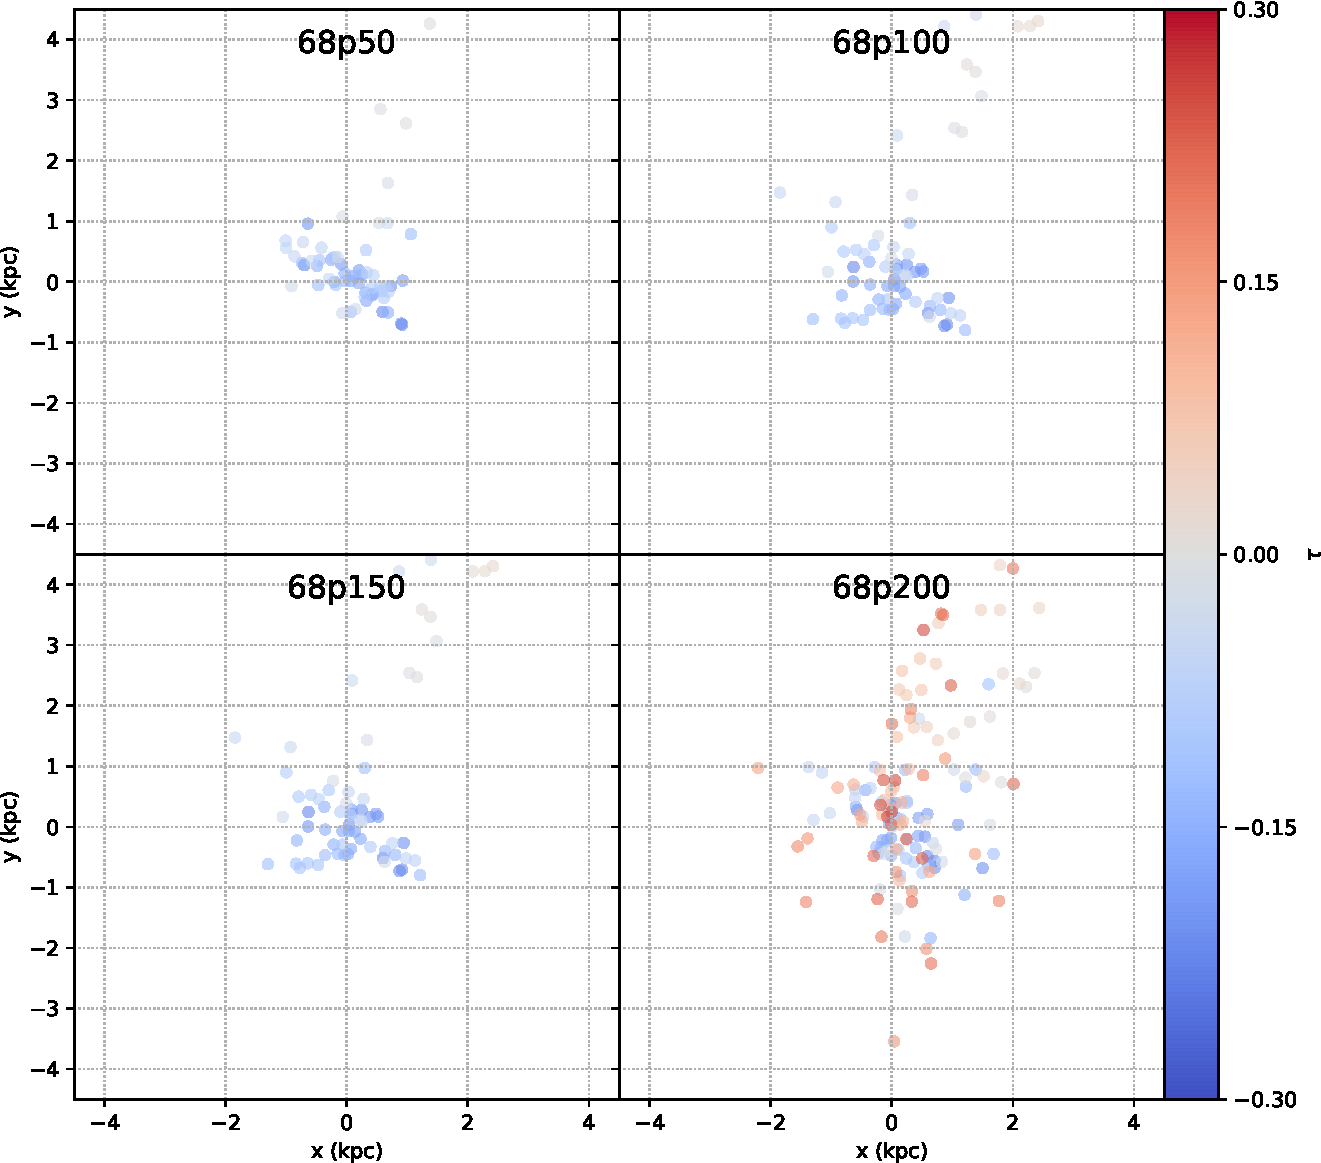
\includegraphics[width=\textwidth]{StarFormationLocation68002.pdf}
\caption{Simulation ID 68}
\end{subfigure}\\[2ex]
\begin{subfigure}[t]{0.7\textwidth}
\centering
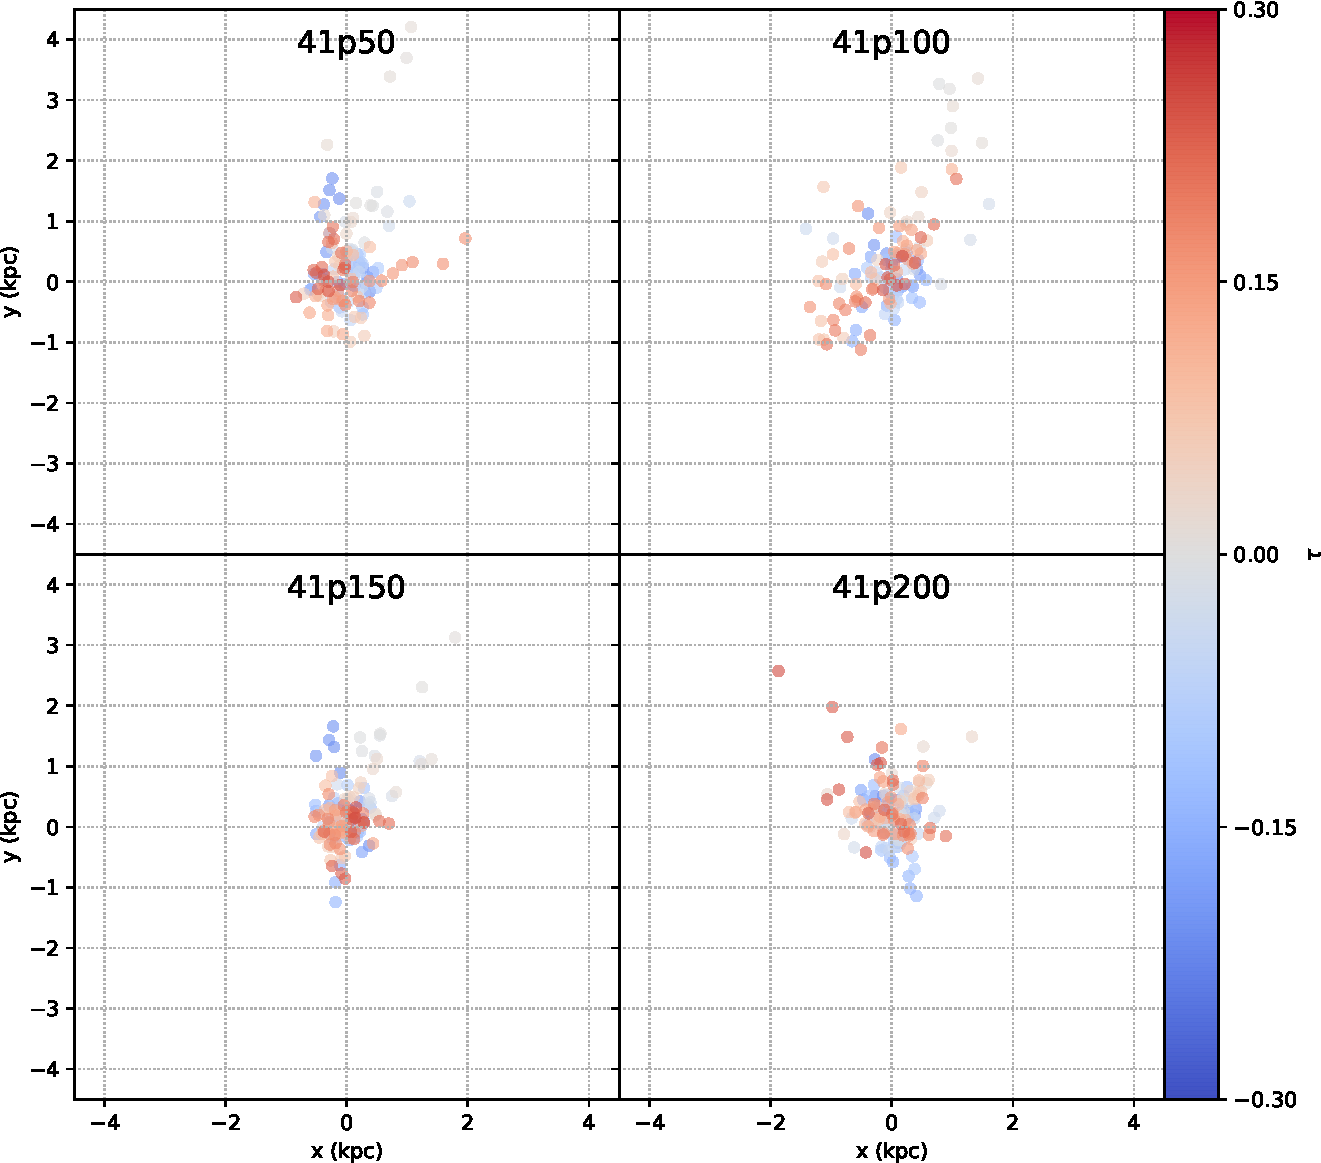
\includegraphics[width=\textwidth]{StarFormationLocation41002.pdf}
\caption{Simulation ID 41}
\end{subfigure}
\caption{Star formation location around first pericenter passage for simulation ID 68 and 41. Each subpanel corresponds to a different pericenter.
The size of the marker is proportional to the number of stars born in that time interval.
Markers are colored using the time from pericenter normalized with the radial period.
In correspondence of pericenter passage an intense star formation activity is registered in the gaseous tail.}
\label{fig:sf_location}
\end{figure*}
In Figure \ref{fig:sf_location} we show the average position of the star forming particles for each simulation snapshot.
For each simulation snapshot the number of new stars w.r.t. to the previous snapshot ($10$~Myr before) is counted and their average position in the $xy$ plane is plotted.
Galaxy is moving in the $-y$ direction (the direction of the instantaneous velocity, see \refsec{sec:MovingBox}) around pericenter.
There is a significant star formation activity in the tail (in Figure~\ref{fig:sf_location}).

An intermediate mass dwarf, ID 68, on orbit of 50 and 100 kpc is completely stripped from the reservoir of cold gas as also shown in the corresponding panel in Figure \ref{fig:cold_gas}. For this, after a burst, star formation stops.

This enforces the idea of the \emph{Jellyfish} phenomenon as a relatively short transitory phase of the galaxy. 


\subsection{Central stellar velocity dispersion}
To start with, we measured the central (within $250$ pc) stellar velocity dispersion for all the simulations on orbit, as shown in Figure~\ref{fig:sigma}.
%Tidal interactions stir the particles in the center of the galaxies. % FIXME  
%TODO There seems to be a bump
% The anisotropy parameter $\beta$ is shown %TODO

\begin{figure}
\centering
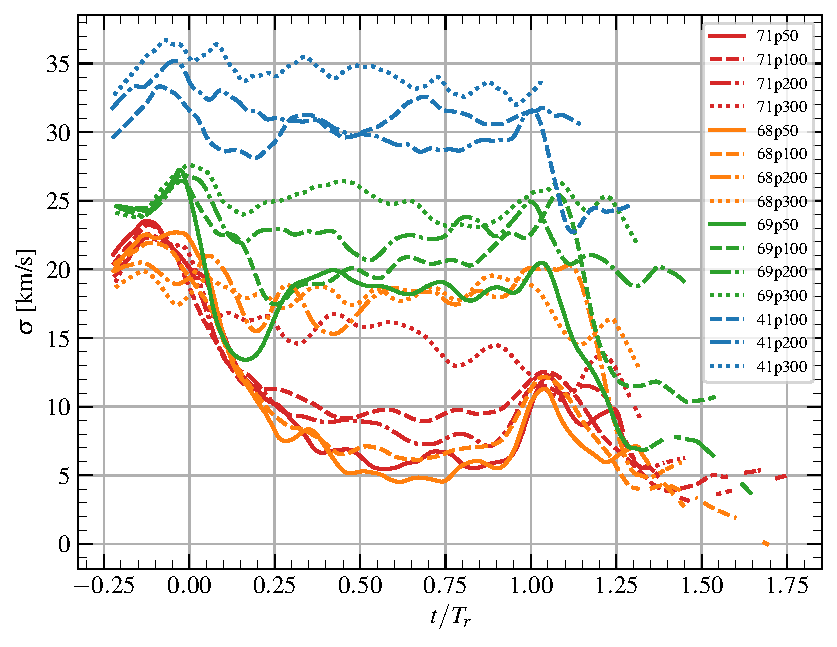
\includegraphics[width=\columnwidth]{fig_sigma_time.pdf}
\caption{Velocity dispersion evolution with time normalised with the radial period of the orbit.
% TODO ADD 150 orbit
}
\label{fig:sigma}
\end{figure}

% \subsection{Stellar metallicity gradients}

%% DERIVED PROPERTIES
\section{Colour Magnitude}
In Figure \ref{fig:g-r} we show the behaviour of the colour magnitude.
In particular the lightest galaxy (ID 62) does not survive the first infall yet ending its life in the early-type galaxy realm, independently of the orbit.
As shown in Figure \ref{fig:cold_gas}, the most massive one (ID 41) retains most of its cold gas except for the most radial orbit.
This is confirmed by its final location on the C-M diagram, among the early-type galaxies.
This allows for star formation to occur almost steadily and to move multiple times between early- and late-type realms.


\begin{sidewaysfigure}
\centering
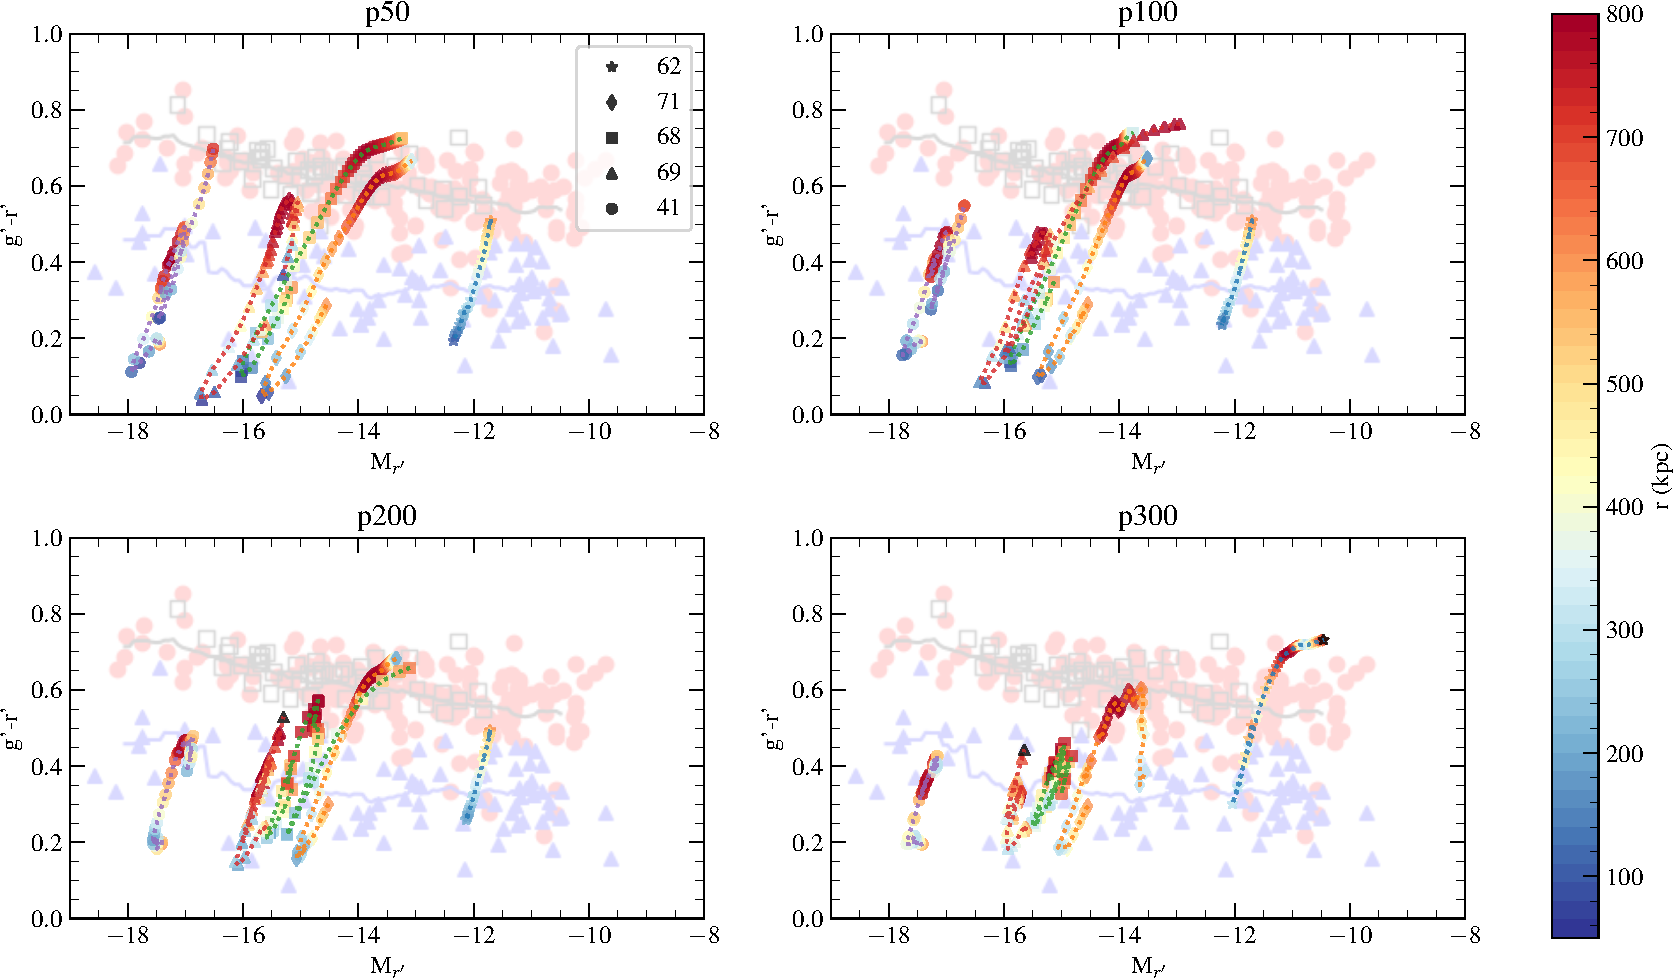
\includegraphics[width=\textwidth]{04.2_color_magnitude_Aku_g-r_rt_criterion_r.pdf}
\caption{SDSS bands colour magnitude diagram of galaxies on different orbits compared to Fornax dwarf catalogue of \citet{Venhola2019}.
% TODO ask permission for the overlay or use catalogue datapoints.
Red and blue colour for the data points in the background represent dwarf elliptical (dE) and late type galaxy respectively, classified by eye on the base of morphology. Empty squares are nucleated dE.
Data tracks of simulated galaxies are shown overlaid colour coded by the clustercentric radius.
The tracks are limited to bound galaxies (i.e. they are drawn with snapshots for which condition \eqref{eq:tidal_radius_condition} holds).
}
\label{fig:g-r}
\end{sidewaysfigure}

\section{HI size mass relation during infall}
\citet{Stevens2019} show how inevitable is the size-mass relation of neutral hydrogen, even during stripping phases.
Our simulations can be checked on the size-mass plane.
As in \citet{Verbeke2017}, we computed the \Hi{} mass by integrating the \Hi{} column density $\Sigma_{\text{\Hi}}$. The radius on the other hand is the major axis of the best fit ellipse on the $1$~\Msun{}~pc$^{-2}$ contour.

%In Figure \ref{fig:hi_size_mass} we show the behaviour of the gas of a representative dwarf.
% We see that our dwarfs stay on the \Hi{} size-mass relation.

\section{Kinematics}
To correctly compute galaxy kinematics we have to take into account the rotation of the moving box.
The details on how to recover the correct in our setup are shown in \refsec{sec:corret_kinematics}.

\subsection{Angular momentum and specific angular momentum}
We compute the specific stellar angular momentum $\lambda_R$ starting from SPH-weighted velocity and velocity dispersion maps as defined in e.g. \citet{Toloba2015}: %TODO add emsellem
\begin{equation}
    \lambda_R = \dfrac{\sum_i F_i R_i |V_i|}{\sum_i F_i R_i \sqrt{V_i^2 + \sigma_i^2}}
\end{equation}
with $i$ the pixel index, $F_i$ its flux and $R_i$ the distance of the pixel from the galaxy center.

% TODO Why this specific form has been chosen. This is what observers like and 

% A typical evolution of $\lambda_R$ through time is shown in Figure~\ref{fig:lambda_R}.
\begin{figure}
\centering
\includegraphics[height=\textheight]{{02.1_lambda_r_vs_js}.pdf}
\caption{Stellar specific angular momentum $\lambda_R$ and specific angular momentum of star particles $j_s$ for the simulation ID 69 on multiple orbits.}
\label{fig:lambda_r_j_s}
\end{figure}

% TODO The relative increase of $\lambda_R$ at first pericenter passage is shown for each orbit and mass in figure \ref{fig:ssam_relative}.
% Around pericenter passages an increase of $\lambda_R$ by a factor of $\approx 2$ is observed.

% \citep{Bidaran2020}

\subsection{Relation with physical angular momentum}
We compute the specific angular momentum ($j_s = J_s/M_g$ where $J_s$ is the total angular momentum and $M_g$ the total mass of the galaxy) of star particles within 10~kpc from the densest stellar region (center of the galaxy).
We compare this specific angular momentum with $\lambda_R$ in Figure \ref{fig:lambda_r_j_s}.
We notice that for example in simulation ID 69, $\lambda_R$ behaviour is very oscillating, quite prone to bursty star formation which can abruptly affect its value.
In our measurements, $\lambda_R$ fails to distinguish pericenter passages unequivocally.
For these reasons in the case of dwarf irregulars it is not a good indicator of the real rotation of the galaxy.
% TODO 41 69 71

\begin{figure}
\centering
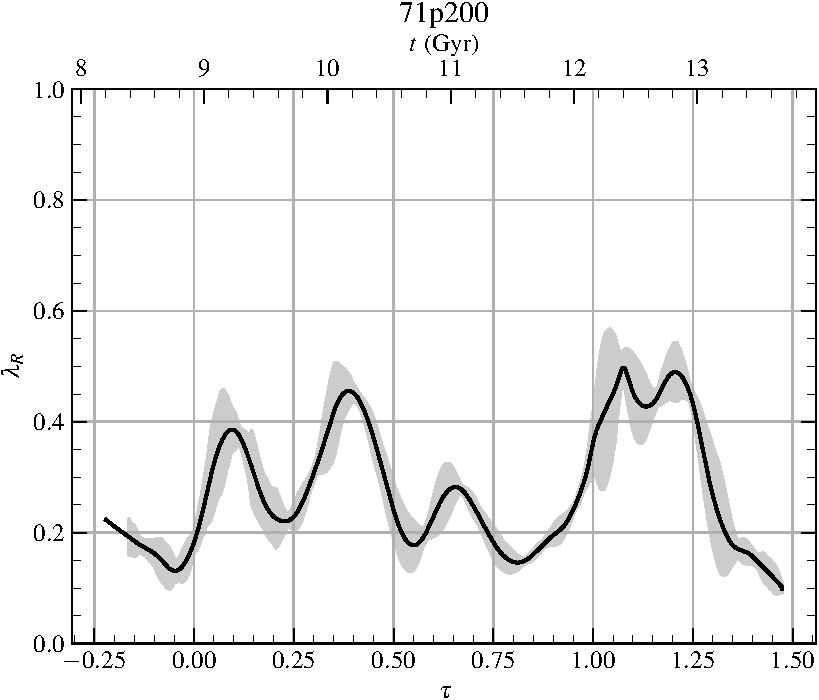
\includegraphics[width=.8\columnwidth]{03.0_fig_lambda_r_time.pdf}
\caption{Specific stellar angular momentum for galaxy ID 71 on a $200$~kpc pericenter orbit.}
\label{fig:lambda_R}
\end{figure}

\section{Conclusion}


% \subsection{Magnitude conversion}
% \pynbody{} can be programmed to compute luminosities of stellar particles using 
% The built in libraries are from Marico... Padova... %TODO
% To obtain SDSS bands we ued conversion formulas from here, after having computed the magnitudes in Johnson bands.
% 
% In particular:

